%%%%%%%%%%%%%%%%%%%%%%%%%%%%%%%%%%%%%%%%%
% Stylish Article
% LaTeX Template
% Version 2.1 (1/10/15)
%
% This template has been downloaded from:
% http://www.LaTeXTemplates.com
%
% Original author:
% Mathias Legrand (legrand.mathias@gmail.com) 
% With extensive modifications by:
% Vel (vel@latextemplates.com)
%
% License:
% CC BY-NC-SA 3.0 (http://creativecommons.org/licenses/by-nc-sa/3.0/)
%
%%%%%%%%%%%%%%%%%%%%%%%%%%%%%%%%%%%%%%%%%

%----------------------------------------------------------------------------------------
%	PACKAGES AND OTHER DOCUMENT CONFIGURATIONS
%----------------------------------------------------------------------------------------

\documentclass[fleqn,10pt]{SelfArx} % Document font size and equations flushed left

\usepackage[italian]{babel} % Specify a different language here - english by default

\usepackage{float}
%----------------------------------------------------------------------------------------
%	COLUMNS
%----------------------------------------------------------------------------------------

\setlength{\columnsep}{0.55cm} % Distance between the two columns of text
\setlength{\fboxrule}{0.75pt} % Width of the border around the abstract

%----------------------------------------------------------------------------------------
%	COLORS
%----------------------------------------------------------------------------------------

\definecolor{color1}{RGB}{0,0,90} % Color of the article title and sections
\definecolor{color2}{RGB}{0,20,20} % Color of the boxes behind the abstract and headings

%----------------------------------------------------------------------------------------
%	HYPERLINKS
%----------------------------------------------------------------------------------------

\usepackage{hyperref} % Required for hyperlinks
\hypersetup{hidelinks,colorlinks,breaklinks=true,urlcolor=color2,citecolor=color1,linkcolor=color1,bookmarksopen=false,pdftitle={Title},pdfauthor={Author}}

%----------------------------------------------------------------------------------------
%	ARTICLE INFORMATION
%----------------------------------------------------------------------------------------

\JournalInfo{Progetto del corso \textit{Industry Lab}, Università degli Studi di Milano Bicocca} % Journal information
\Archive{Anno Accademico 2019-20} % Additional notes (e.g. copyright, DOI, review/research article)

\PaperTitle{GP5 - Analisi dei dati e previsione del coefficiente di perdita} % Article title

\Authors{Riccardo Cervero\textsuperscript{1}, Marco Savino\textsuperscript{2}, Luca Lazzati\textsuperscript{3}} % Authors
\affiliation{\textsuperscript{1}\textit{794126, Dipartimento di Informatica, Sistemistica e Comunicazione}} % Author affiliation
\affiliation{\textsuperscript{2}\textit{793516, Dipartimento di Informatica, Sistemistica e Comunicazione}} % Author affiliation
\affiliation{\textsuperscript{3}\textit{?, Dipartimento di Informatica, Sistemistica e Comunicazione}}

\Keywords{Monitoraggio -- Previsione} % Keywords - if you don't want any simply remove all the text between the curly brackets
\newcommand{\keywordname}{Keywords} % Defines the keywords heading name

%----------------------------------------------------------------------------------------
%	ABSTRACT
%----------------------------------------------------------------------------------------

\Abstract{}

%----------------------------------------------------------------------------------------

\begin{document}

\flushbottom % Makes all text pages the same height

\maketitle % Print the title and abstract box

\tableofcontents % Print the contents section

\thispagestyle{empty} % Removes page numbering from the first page

%----------------------------------------------------------------------------------------
%	ARTICLE CONTENTS
%----------------------------------------------------------------------------------------

\section*{Caso di studio} % The \section*{} command stops section numbering

\addcontentsline{toc}{section}{Caso di studio} 

%Spiegazione problema

%------------------------------------------------
\section{Data Preparation}
Il \textit{database} si compone di 296605 osservazioni, descritte da 33 colonne. Tuttavia, è stato necessario focalizzare l'analisi su quelle che presentavano un certo grado di rilevanza e utilità per l'oggetto di studio. Ciò ha comportato la rimozione, durante una prima fase di \textit{pre-processing}, delle variabili che presentavano le seguenti caratteristiche: si manifestavano come un unico valore costante\footnote{Le costanti rimosse sono: \texttt{"Banco"}, \texttt{"Master"}, \texttt{"Picco coppia zero"}, \texttt{"Picco coppia iniziale"}, \texttt{"Media coppia iniziale"}, \texttt{"Velocità 1"}, \texttt{"Picco pressione velocità 2"}, \texttt{"Media pressione velocita 2"}, \texttt{"Picco portata velocità 2"}, \texttt{"Media portata velocità 2"}.}, mostravano una distribuzione eccessivamente sbilanciata verso una sola classe\footnote{È questo il caso di \texttt{"Velocità 2"}, \texttt{"Esito"} e di conseguenza \texttt{"N. Esito"}, \texttt{"Coppia max ciclo"}, \texttt{"Velocità a regime"}.}, erano ridondanti, poco interessanti o erano già state segnalate tali dai fornitori del \textit{dataset}\footnote{Le colonne inutili sono: \texttt{"Codice da Linea"} - identificativo del pezzo -, \texttt{"Media coppia zero"}, \texttt{'Data'} e \texttt{'Ora'}, poiché i dati sono stati raccolti in un arco temporale non uniforme.}. Infine, è stata rimossa una sola riga, poiché penalizzata dalla mancanza dei valori di pressione.
%------------------------------------------------
\section{Analisi preliminari}
Dopo le operazioni di pulizia appena menzionate, si è proceduto ad analizzare in maniera preliminare le colonne rilevanti, per ottenere un primo approfondimento sui descrittori e i rapporti di dipendenza fra gli stessi. 
\subsection{Variabili categoriche}
I dati nominali conservati sono relativi a due precisi aspetti del processo: la segmentazione del lavoro in turni differenti e il programma selezionato per la creazione del pezzo, ovvero la tiplogia di pompa.\\
Per quanto riguarda la prima, è stato necessario aggregare le medesime classi registrate erroneamente in maniera diversa, uniformandone la denominazione. In questo modo, sono state ottenute 5 classi: "A", "B", "C", "D", "0". Le ultime due sono state osservate in minor misura e non specificate inizialmente dai fornitori del \textit{dataset}, e pertanto etichettate come "\textit{non valori}".
\begin{figure}[h]
    \centering
    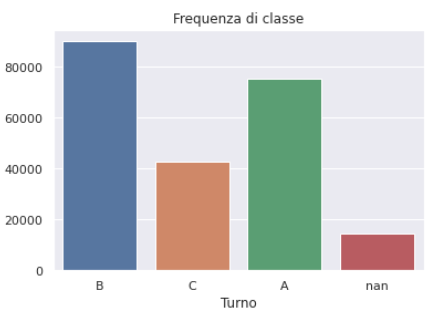
\includegraphics[width=0.9 \linewidth]{turno.png}
    \label{fig:em}
    \caption{\textit{Bar chart} per la visualizzazione delle rispettive frequenze osservate dei turni.}
\end{figure}
Come osservabile in Figura 1, i principali blocchi in cui è organizzato il processo presentano una frequenza diversa: il turno "B" costituisce più del 40\% dei \textit{records}, "A" si presenta nel $\sim$34\% dei casi e "C" nel $\sim$19\%.\\
La composizione del "Programma" mostra un fortissimo sbilanciamento verso la classe GP5 denominata \texttt{18\_GP5\_910\_CW} (Figura 2), che corrisponde alla pompa "\textit{Daimler}". Le restanti tipologie, raggruppate sotto denominazione "Standard", formano in totale meno del 23\% dei casi e sono principalmente rappresentate dalle categorie \texttt{17\_GP5\_430\_CCW} (10.6\%) e \texttt{12\_GP5\_430B\_D1} (8.5\%).
\begin{figure}[h]
    \centering
    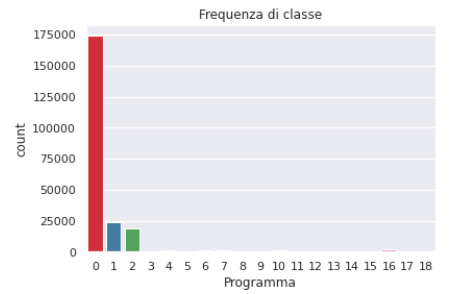
\includegraphics[width=0.9 \linewidth]{prog.png}
    \label{fig:em}
    \caption{\textit{Bar chart} per la visualizzazione delle rispettive frequenze osservate dei programmi.}
\end{figure}
Per una visualizzazione migliore, in Figura 3 è riassunta la distribuzione delle frequenze logaritmiche delle varie classi GP5.
\begin{figure}[h]
    \centering
    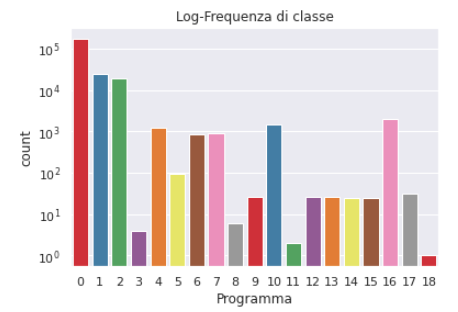
\includegraphics[width=0.9 \linewidth]{proglog.png}
    \label{fig:em}
    \caption{\textit{Bar chart} per la visualizzazione delle rispettive frequenze logaritmiche dei programmi.}
\end{figure}
Tra le variabili categoriche esaminate, "Esito" descrive le eventuali - rarissime - imperfezioni del prodotto. A tal proposito, il 99.5\% delle volte, il risultato è ottimale, mentre l'anomalia più comune è indicata come "scarto picco coppia max fase pulizia iniziale" (0.1\% delle osservazioni).
\subsection{Variabili numeriche}
I dati numerici registrano, per ogni pompa, due principali set di valori, relativi al picco e alla media rispettivamente di pressione (in bar) e portata (in litri all'ora), misurati in corrispondenza di due velocità diverse:
\begin{itemize}
    \item a regime: 2300 \textit{r.p.m}
    \item 140 \textit{r.p.m}
\end{itemize}
Si vedrà che, a prescindere dalla velocità, le due grandezze condividono un'elevatissima dipendenza lineare.
\subsubsection{Descrittori della pressione}
Innanzitutto, le grandezze relative al picco e alla media hanno una distribuzione multimodale nell'ambito di entrambe le misurazioni della velocità (Figura 4), rivelando picchi di diversa altezza. Il range osservato è molto superiore per quanto concerne la velocità a regime (come riassunto dalla Tabella 1). Inoltre, le distribuzioni dei valori appaiono quasi identiche per classe di velocità, rivelando una fortissima similarità fra l'andamento del picco e e della pressione media (Figura 5).
\begin{figure}[h]
    \centering
    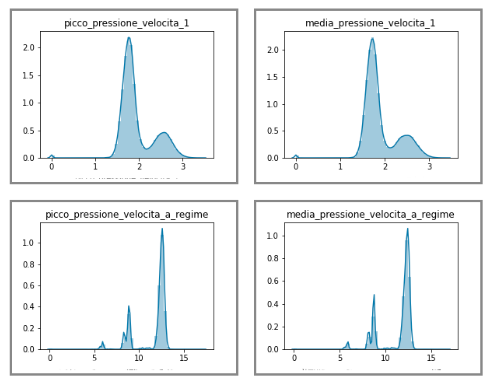
\includegraphics[width=1 \linewidth]{press.png}
    \label{fig:em}
    \caption{Distribuzioni delle grandezze relative alla pressione.}
\end{figure}
\begin{figure}[h]
    \centering
    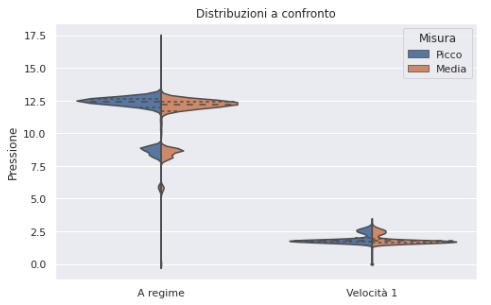
\includegraphics[width=1 \linewidth]{p.png}
    \label{fig:em}
    \caption{Distribuzioni delle grandezze relative alla pressione, in corrispondenza della velocità "1" e a regime, appaiate nell'ambito della stessa misurazione. È possibile notare sia la superiorità della pressione a regime, che la fortissima vicinanza dell'andamento del picco rispetto alla pressione media.}
\end{figure}
{\begin{table}[h]
\centering
\begin{tabular}[t]{lccc}
\toprule
Pressione&Minimo&Media&Massimo\\
\midrule
\textbf{Picco (140)}&0.19&1.94&3.45\\
\textbf{Picco (2300)}&5.38&11.61&14.21\\
\textbf{Media (140)}&0.1&1.88&3.38\\
\textbf{Media (2300)}&5.33&11.41&14.01\\
\bottomrule
\end{tabular}
\caption{Rassunto relativo alla media e al range dei valori di pressione.}
\end{table}}
\subsubsection{Descrittori della portata}
Le rispettive distribuzioni di portata (Figura 6) rivelano andamenti molto meno regolari. In particolare, i \textit{records} a regime sono caratterizzati da una coda molto estesa verso destra, lasciando presupporre la presenza di una  quota rilevante di valori anomali e permettendo di intravedere una ancor più forte differenza rispetto a quanto visibile con una velocità pari ai 140 \textit{r.p.m}.  
\begin{figure}[h]
    \centering
    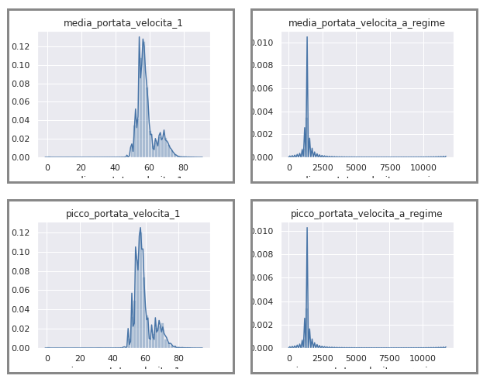
\includegraphics[width=1 \linewidth]{port.png}
    \label{fig:em}
    \caption{Distribuzioni delle grandezze relative alla portata.}
\end{figure}
{\begin{table}[h]
\centering
\begin{tabular}[t]{lccc}
\toprule
Portata&Minimo&Media&Massimo\\
\midrule
\textbf{Picco (140)}&30.30&58.96&93.6\\
\textbf{Picco (2300)}&930.5&1309.6&1422.9\\
\textbf{Media (140)}&28.07&58.5&90\\
\textbf{Media (2300)}&927.63&1304.8&1416.2\\
\bottomrule
\end{tabular}
\caption{Rassunto relativo alla media e al range dei valori di portata.}
\end{table}}
I comportamenti mostrati dalle osservazioni relative alla pressione della pompa si ritrovano in forma identica esaminando le misurazioni di portata: anche qui, esiste una grandissima somiglianza fra le distribuzioni di picco e media, e - come anticipato - una differenza di scala ancor più ampia fra i valori estratti per le due velocità (Figura 7).
\begin{figure}[H]
    \centering
    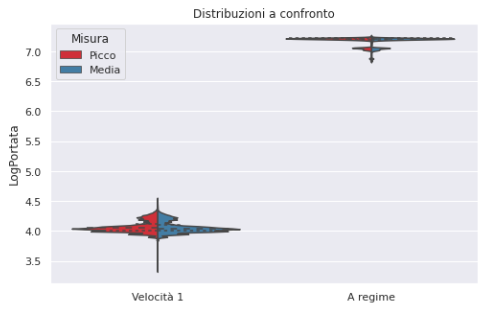
\includegraphics[width=1 \linewidth]{port2.png}
    \label{fig:em}
    \caption{Distribuzioni delle grandezze relative alla portata, in corrispondenza della velocità "1" e a regime, appaiate nell'ambito della stessa misurazione. Poichè la differenza era troppo grande per permettere una visualizzazione comprensibile, è stato necessario adottare una scala logaritmica.}
\end{figure}
Infine, è interessante notare come le colonne relative alla pressione e alla portata condividano reciproce dipendenze lineari con grado molto elevato, come visibile in Figura 8: la correlazione assoluta media raggiunge addirittura un livello di $\sim$0.95, con un minimo di 0.79 - tra i picchi di portata misurati fra le due velocità - e 8 collinearità perfette. In particolare, oltre alla quasi identicità delle distribuzioni nell'ambito della stessa grandezza - menzionata in precedenza - appaiono interessanti le seguenti dipendenze lineari:
\begin{itemize}
    \item picco pressione e picco portata, entrambi alla velocità di 140 \textit{r.p.m.} ($\sim$0.91)
    \item media pressione e picco portata, sempre per quanto riguarda la fase di controllo \textit{r.p.m.} ($\sim$0.91)
    \item media portata e picco pressione, a 140 \textit{r.p.m.} ($\sim$0.92)
    \item media portata e media pressione, per la fase di controllo ($\sim$0.92)
    \item media pressione e media portata a velocità di regime, fra cui s'individua una correlazione perfetta
    \item picco pressione e picco portata a velocità di regime, sempre una correlazione perfetta
    \item picco portata e media pressione a velocità di regime: perfetta collinearità.
\end{itemize}
\begin{figure}[H]
    \centering
    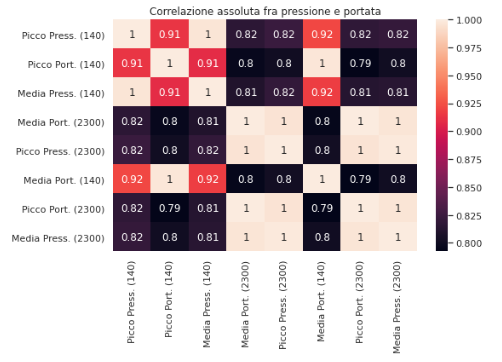
\includegraphics[width=1 \linewidth]{corrpp.png}
    \label{fig:em}
    \caption{Matrice di correlazione, con valori assoluti, fra tutte le variabili di pressione e portata.}
\end{figure}
Appare quindi evidente la sistematica dipendenza fra pressione e portata, che, osservando i dati forniti, paiono spesso essere state generate dalla stessa distirbuzione casuale, a prescindere dalla misura scelta e dalla fase impostata. Per questa ragione, in fase di generazione dei modelli di regressione, la matrice del disegno potrebbe essere affetta da un eccessivo problema di multicollinearità, rischiando di divenire singolare o addirittura non invertibile, penalizzando una stima corretta sia dei coefficienti di regressione che degli indici di bontà di adattamento della funzione di regressione. Sarà pertanto necessario rimuovere tali variabili più correlate, oppure adottare strategie utili alla selezione di un modello a più bassa dimensionalità, come, ad esempio, le tipologie \textit{Ridge} e \textit{LASSO}.
\subsubsection{Altre variabili}
Le altre colonne numeriche, filtrate dalla fase di \textit{pre-processing} e ritenute rilevanti ai fini dello studio, sono: media coppia in fase finale (100 \textit{rpm}), picco coppia in fase finale e temperatura di prova del liquido.\\
Per quanto riguarda la prima, la distribuzione è fortemente asimmetrica verso valori elevati, con una discreta porzione di \textit{outliers}. Il picco della stessa grandezza presenta una coda ancor più lunga (in scala logaritmica in Figura 9). Medesima condizione di elevata asimmetria vale per la temperatura, compresa fra un range di 37.61° e 49.1°.
\begin{figure}[h]
    \centering
    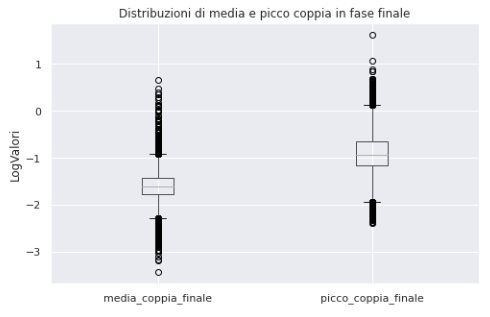
\includegraphics[width=1 \linewidth]{cf.png}
    \label{fig:em}
    \caption{\textit{Boxplot} per la visualizzazione della distribuzione delle variabili "Media coppia finale" e "Picco coppia finale".}
\end{figure}
È importante citare che anche fra la media e il picco della coppia in fase finale (100 \textit{rpm}) esista una forte dipendenza lineare positiva ($\sim$0.83). Bisognerà pertanto valutare questa ulteriore collinearità in fase di stima del modello per la previsione del coefficiente.\\
Al contrario, queste due variabili non presentano un'elevata dipendenza rispetto i dati di pressione e portata: la correlazione rimane sempre ben al di sotto del 20\%. Lo stesso vale per i valori di temperatura.

\subsection{Target: coefficiente di dispersione}
Il coefficiente di dispersione è calcolato con la formula
$$\alpha=\frac{108.36-\text{Media portata (@140)}}{\text{Media pressione (@140)}}$$.

%Distribuzione
%Correlazione
%Programma
%No serie storica

\subsection{\textit{Outliers Detection}}
%------------------------------------------------
\section{Sistema di monitoraggio \textit{real-time}}
%------------------------------------------------
\section{Limite dinamico di portata}
%----------------------------------------------------------------------------------------
\section{Modelli di previsione}
%----------------------------------------------------------------------------------------
%	REFERENCE LIST
%----------------------------------------------------------------------------------------
\phantomsection
\bibliographystyle{unsrt}
\bibliography{sample}

%----------------------------------------------------------------------------------------

\end{document}
